\documentclass[dvipdfmx]{beamer}
\usepackage{tutorial}

\title{計算機実験(L7) --- 最適化問題・スーパーコンピューターと計算物理}
\date{2016/06/29}

\begin{document}

\begin{frame}
  \titlepage
  \tableofcontents
\end{frame}

\section{最適化問題}

\begin{frame}[t,fragile]{最適化問題}
  \begin{itemize}
    %\setlength{\itemsep}{1em}
  \item 目的関数$f(x)$の最小値(あるいは最大値)とその場所を求めたい
    \begin{itemize}
    \item 連続最適化問題
    \item 離散最適化(組み合わせ最適化)問題 $\Leftarrow$ 難しい
    \end{itemize}
  \item 真の(大局的な)最小値(最大値)を求めるのは難しい
  \item 一般的には極値を求めることしかできない
  \item 多次元では極小を囲い込むことができない
  \item 導関数を使う方法: ニュートン法、最急降下法、勾配降下法, 共役勾配法、準ニュートン法
  \item 使わない方法: 囲い込み法、Nelder-Meadの滑降シンプレックス法、シミュレーテッド・アニーリング
  \end{itemize}
\end{frame}

\input{72_descent.tex}
\section{最適化手法の比較}

\begin{frame}[t,fragile]{例題 (二次元の最適化)}
  \begin{center}
    \resizebox{.9\textwidth}{!}{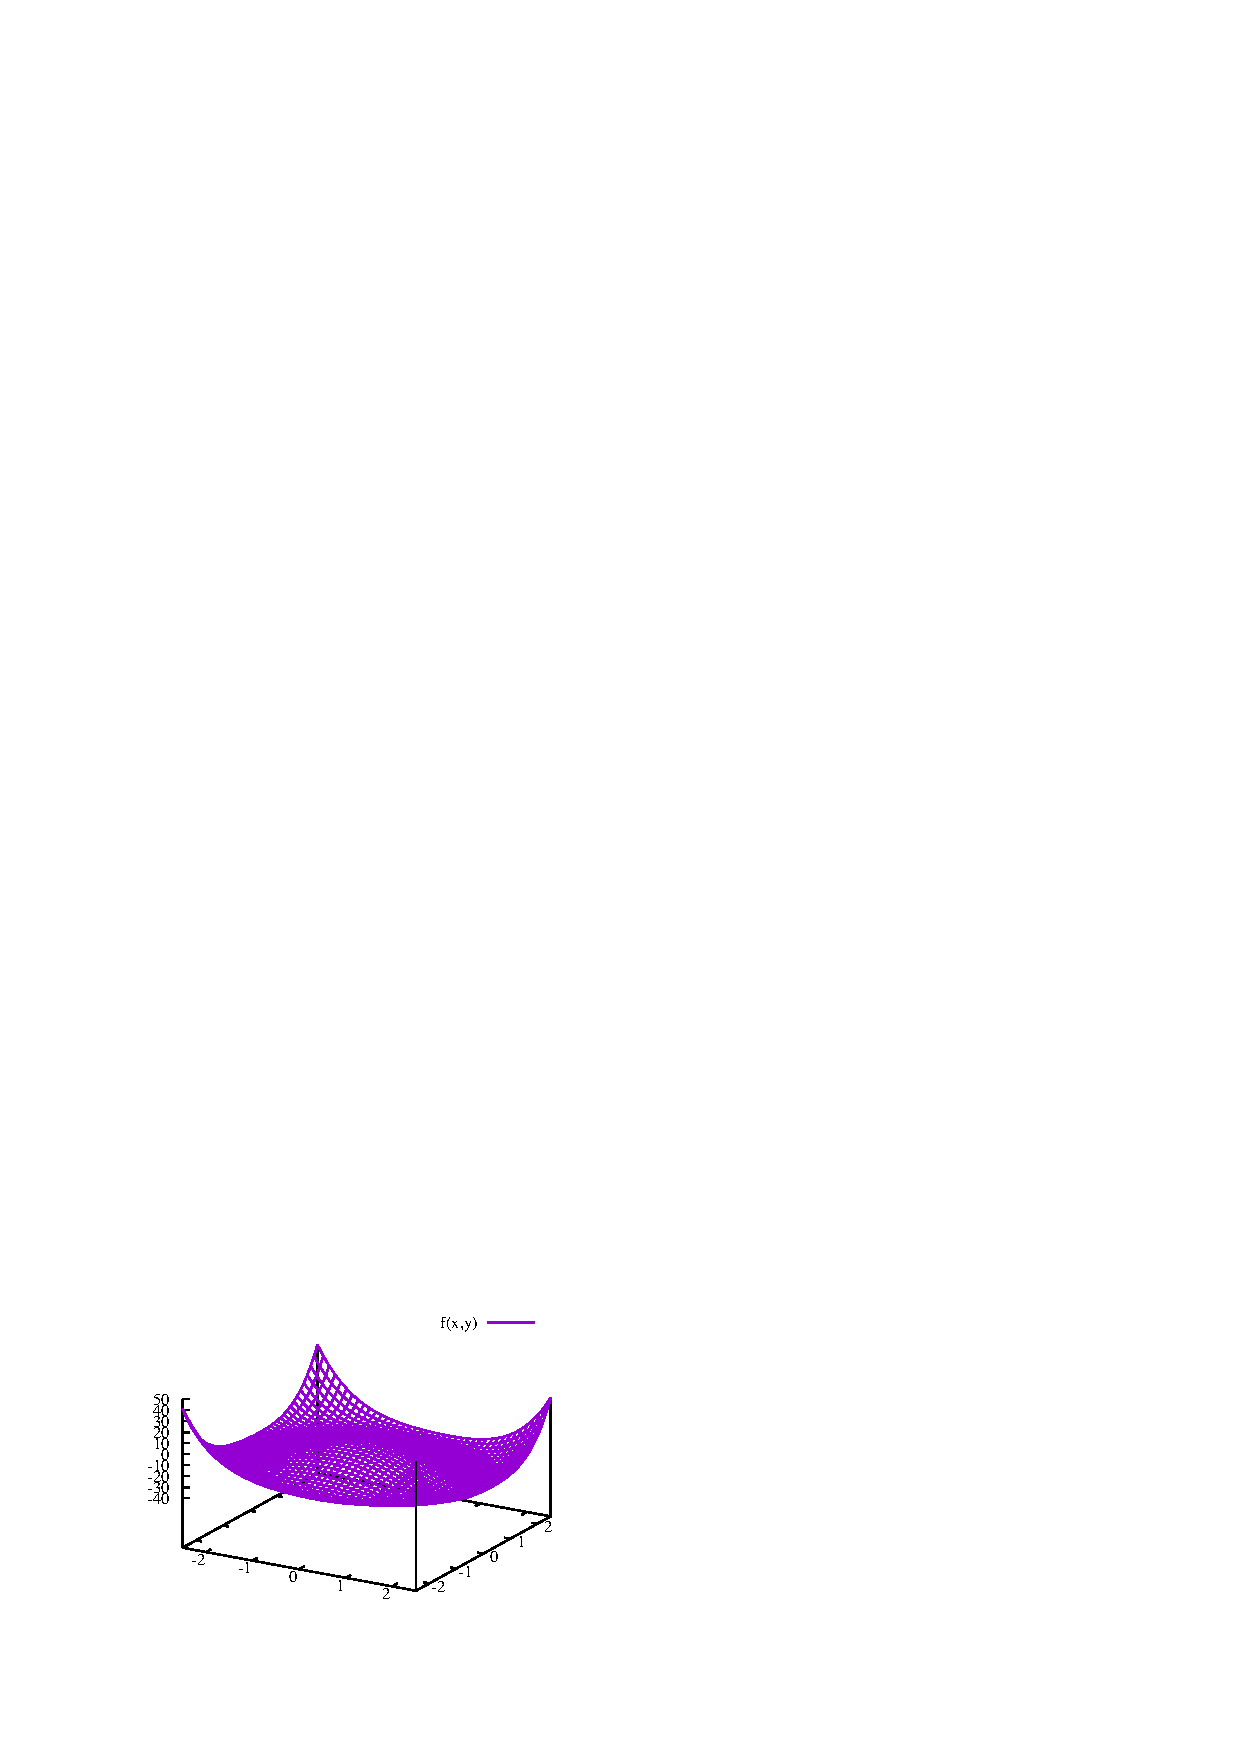
\includegraphics{image/func_2d.pdf}}
  \end{center}
\end{frame}

\begin{frame}[t,fragile]{様々な最適化手法の比較 (1/4)}
  \begin{center}
    \resizebox{.9\textwidth}{!}{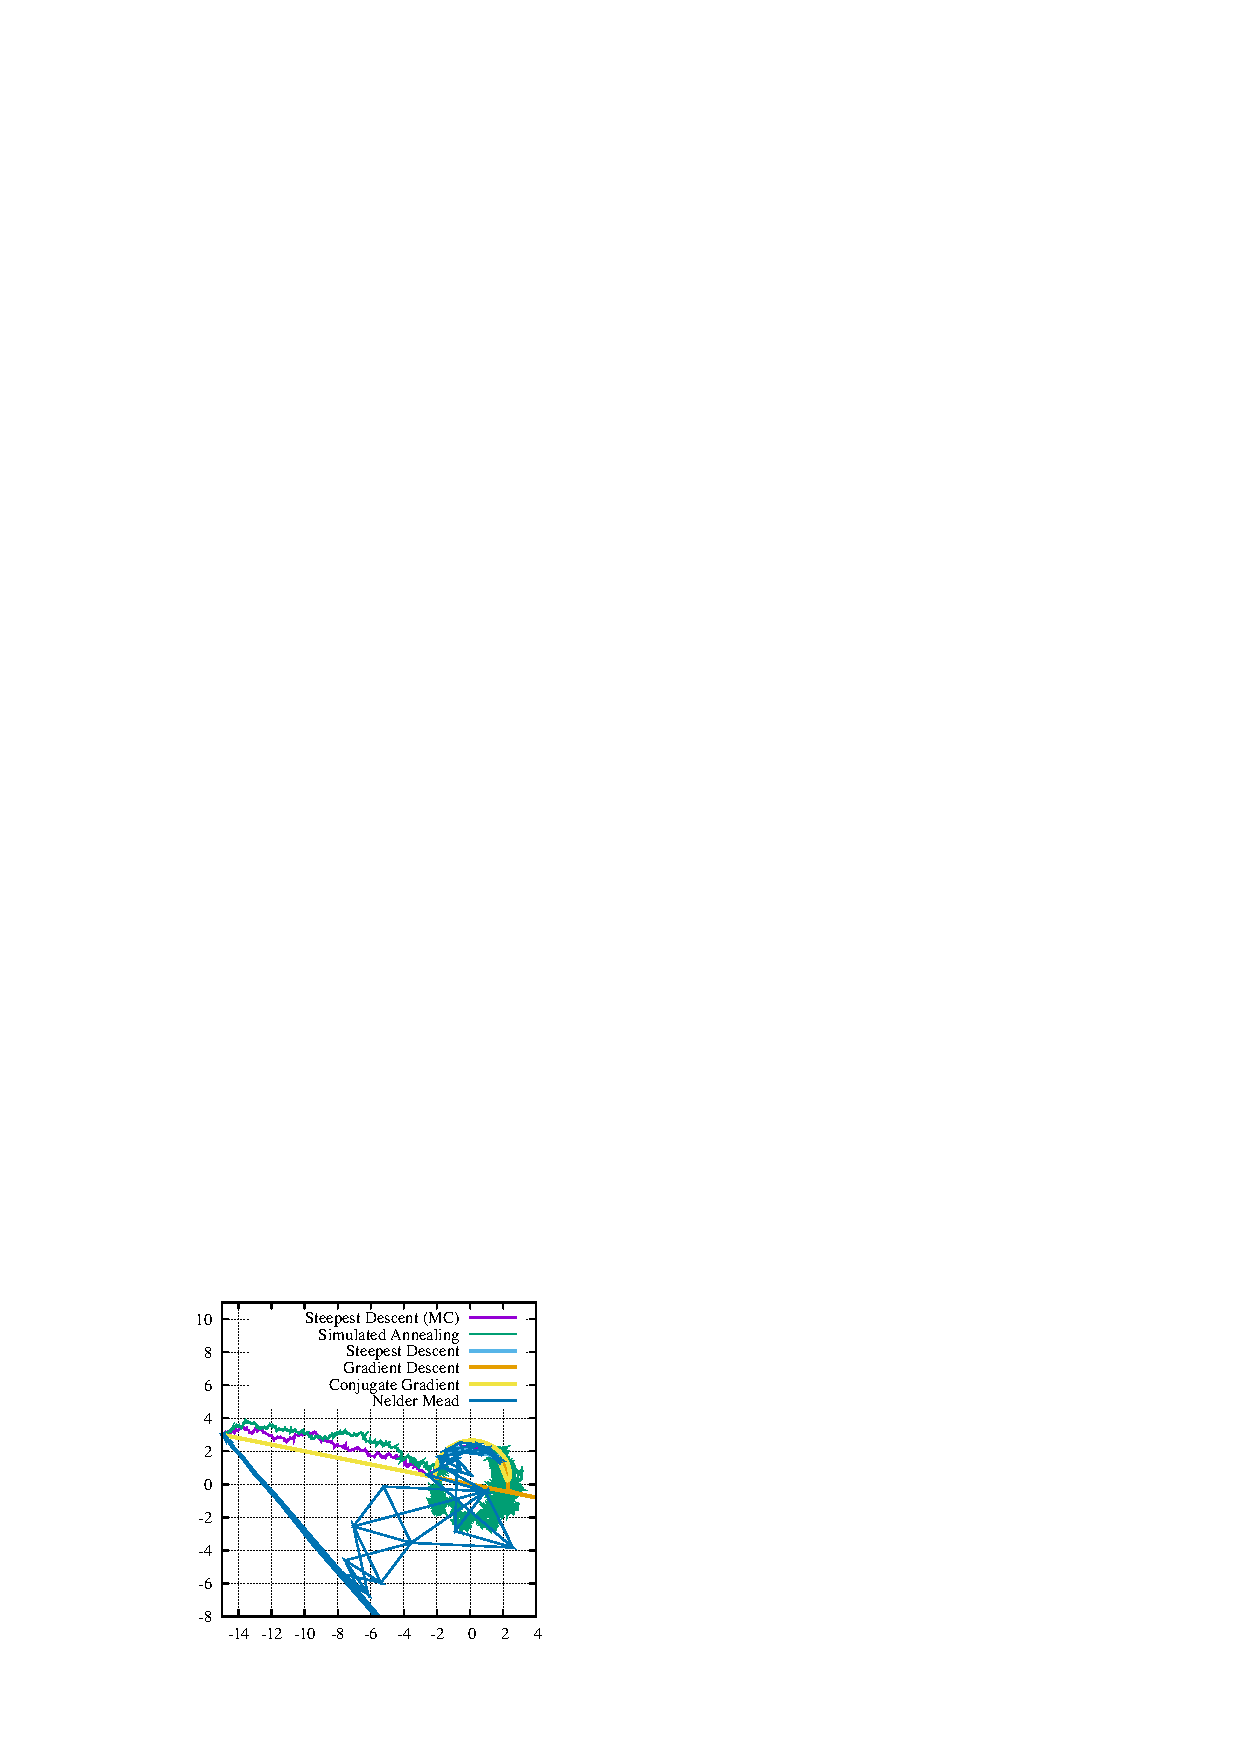
\includegraphics{image/optimization.pdf}}
  \end{center}
\end{frame}

\begin{frame}[t,fragile]{様々な最適化手法の比較 (2/4)}
  \begin{center}
    \resizebox{.9\textwidth}{!}{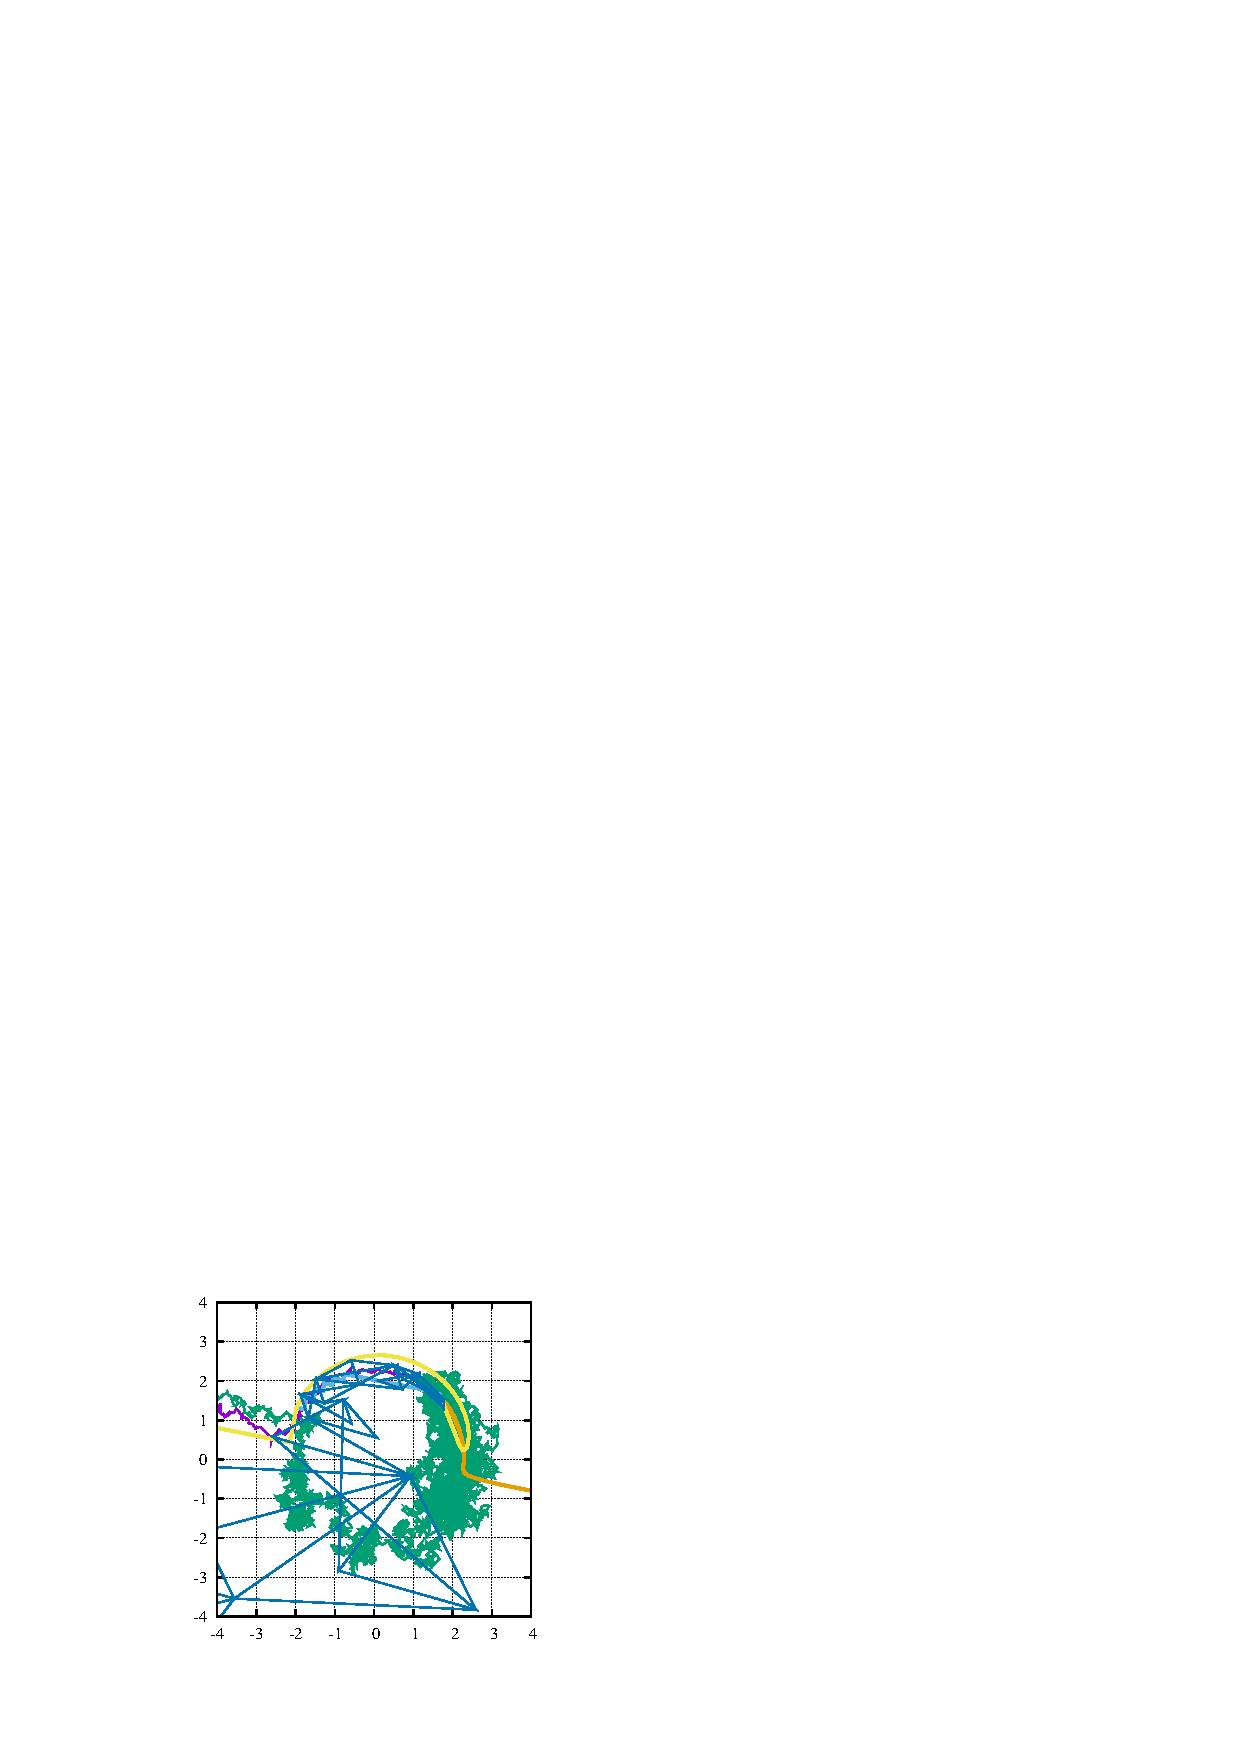
\includegraphics{image/optimization2.pdf}}
  \end{center}
\end{frame}

\begin{frame}[t,fragile]{様々な最適化手法の比較 (3/4)}
  \begin{center}
    \resizebox{.9\textwidth}{!}{\includegraphics{image/optimization3.pdf}}
  \end{center}
\end{frame}

\begin{frame}[t,fragile]{様々な最適化手法の比較 (4/4)}
  \begin{center}
    \resizebox{.9\textwidth}{!}{\includegraphics{image/optimization4.pdf}}
  \end{center}
\end{frame}

\section{スーパーコンピューターと計算物理}

\begin{frame}[t,fragile]{計算機の進化}
  \begin{itemize}
    \setlength{\itemsep}{1em}
  \item 計算機の性能は指数関数的に伸び続けている
    \begin{itemize}
    \item 1年で1.9倍 ⇒ 4年で10倍 ⇒ 過去70年間で100兆倍
    \item 世界初のスパコンCray-1 (1976年)の演算性能 約160MFlops
    \item iPhone6 (2014年)の演算性能 約900MFlops
    \item 2020年代初頭には、1EFlops (エクサフロップス)へ
    \end{itemize}
  \item 現代のスーパーコンピュータは全て
    \begin{itemize}
      \item 並列コンピュータ (CPU数 1,000〜100,000)
      \item マルチコア or メニーコア (CPUあたりのコア数 8 〜 1,000)
      \item 多層にわたる階層構造
      \item 演算に比べて、データを移動するコストの方が高い
    \end{itemize}
  \end{itemize}
\end{frame}

\input{81_parallel.tex}
\section{バッチキューシステム}

\begin{frame}[t,fragile]{バッチキューシステム}
  \begin{itemize}
    \setlength{\itemsep}{1em}
  \item 実習用計算機 photon
    \begin{itemize}
    \item ログインノード(2CPU, 12コア)+計算ノード(64CPU, 256コア)からなる「クラスタワークステーション」(並列計算機の一種)
    \item 普段{\tt ssh}して作業しているのはログインノード
    \end{itemize}
  \item バッチーキューシステム
    \begin{itemize}
    \item 長い(大きな)計算は計算ノードを使う
    \item 多数の計算ノードの割り振りを手でやるのは非効率的
    \item バッチキューシステムを使って、「ジョブ」を投入する
    \end{itemize}
  \item 詳しい説明は「システム利用マニュアル」({\tt ssh}ログイン時に表示されるメッセージ参照)を見ること
  \item photon は卒業まで継続して利用可 (希望すれば大学院でも)
  \end{itemize}
\end{frame}


\section{}

\begin{frame}[t,fragile]{実習・講義予定}
  \begin{itemize}
    \setlength{\itemsep}{1em}
  \item 実習 EX6
    \begin{itemize}
    \item モンテカルロ法
    \item 最適化
    \item レポートNo.3: 締切7/29(金)
    \end{itemize}
  \item 7/13 グループワーク発表会
    \begin{itemize}
    \item タイトル・ライトニングトーク用スライド(PPT・1枚): 締切7/12(火)
    \item ポスター掲示(1220室前のロビー): 7/13(水) 10:15-10:25
    \item ライトニングトーク: 10:25-11:00 (各グループ2分以内)
    \item ポスターセッション: 11:00-12:10
    \item グルプーレポート: ポスター(を修正したもの)を提出。締切7/15(金)
    \item 発表会に関する連絡事項等はITC-LMSに掲載するので、適宜確認すること
    \end{itemize}
  \end{itemize}
\end{frame}

\end{document}
